\documentclass[
  11pt,
  letterpaper,
  % addpoints,
   answers
  ]{exam}
\usepackage{float}
\usepackage{../exercise-preamble}

\begin{document}

\noindent
\begin{minipage}{0.47\textwidth}
  
\includegraphics[width=\textwidth]{../fcfm_die}
\end{minipage}
\begin{minipage}{0.53\textwidth}
\begin{center} 
\large\textbf{Electromagnetismo Aplicado} (EL3103) \\
\large\textbf{Clase auxiliar 1} \\
\normalsize Prof.~\professor\\
\normalsize Prof. Aux. Lucas Palomino
\\
\normalsize Ayudantes: \ayudanteA~-~\ayudanteB
\end{center}
\end{minipage}

\vspace{0.5cm}
\noindent
\vspace{.85cm}

\section{Resumen:}

Sea $f$ un campo escalar de clase $\mathcal{C}^2$, se define el \textbf{operador Laplaciano} como:
\[
\nabla^2 f = \nabla \cdot (\nabla f)
\]
o, equivalentemente, como la suma de las segundas derivadas parciales de $f$ en el sistema de coordenadas correspondiente:

\begin{itemize}
    \item \textbf{Coordenadas cartesianas} $(x,y,z)$:
    \[
    \nabla^2 f = \frac{\partial^2 f}{\partial x^2}
               + \frac{\partial^2 f}{\partial y^2}
               + \frac{\partial^2 f}{\partial z^2}
    \]

    \item \textbf{Coordenadas cilíndricas} $(r,\phi,z)$:
    \[
    \nabla^2 f = \frac{1}{r} \frac{\partial}{\partial r}
    \left( r \frac{\partial f}{\partial r} \right)
    + \frac{1}{r^2} \frac{\partial^2 f}{\partial \phi^2}
    + \frac{\partial^2 f}{\partial z^2}
    \]

    \item \textbf{Coordenadas esféricas} $(r,\theta,\phi)$:
    \[
    \nabla^2 f =
    \frac{1}{r^2} \frac{\partial}{\partial r}
    \left( r^2 \frac{\partial f}{\partial r} \right)
    + \frac{1}{r^2 \sin\theta} \frac{\partial}{\partial \theta}
    \left( \sin\theta \frac{\partial f}{\partial \theta} \right)
    + \frac{1}{r^2 \sin^2\theta} \frac{\partial^2 f}{\partial \phi^2}
    \]
\end{itemize}

\subsection*{Ecuaciones de Poisson y Laplace}

A continuación, se enuncian dos expresiones fundamentales para el desarrollo de los problemas posteriores.  
La primera corresponde a la \textbf{ecuación de Poisson}, que se expresa como:

\begin{equation}
\nabla^{2} V = -\frac{\rho}{\varepsilon_{0}}
\end{equation}

donde:
\begin{itemize}
    \item $V$ es el \textit{potencial eléctrico}.
    \item $\rho$ es la densidad de carga total, incluyendo tanto carga libre ($\rho_f$), como carga ligada ($\rho_b$).
    \item $\varepsilon_{0}$ es la permitividad del vacío.
\end{itemize}

En el caso particular en que el medio no contenga densidad de carga ($\rho = 0$), la ecuación de Poisson se reduce a la \textbf{ecuación de Laplace}:

\begin{equation}
\nabla^{2} V = 0
\end{equation}

\subsection*{Propiedades de la ecuación de Laplace}
La ecuación de Laplace cumple las siguientes características:
\begin{itemize}
    \item \textbf{La media es el promedio de los extremos.}
    \item \textbf{La ecuación de Laplace no tolera mínimos ni máximos globales.} Es decir, el valor máximo y valor mínimo del potencial se encontrarán en los extremos.
    \item \textbf{La solución a la ecuación de Laplace es única.}
    \item \textbf{La ecuación de Laplace es lineal.}
\end{itemize}
\subsection*{Ecuaciones de Maxwell en electroestática y magnetoestática}
\begin{align}
  \text{(i)}&\quad \tcbhighmath{\nabla\cdot \mathbf{E}= \frac{\rho}{\epsilon_0}} & \text{(iii)}&\quad \tcbhighmath{\nabla\times \mathbf{E} = 0}\\
  \text{(ii)}&\quad \tcbhighmath{\nabla\cdot \mathbf{B} = 0} & \text{(iv)}&\quad \tcbhighmath{\nabla\times \mathbf{B} = \mu_0 \cdot \mathbf{J}}
  \end{align}
  Además, se tendrán las siguientes relaciones útiles:
  \begin{align}
      \quad \tcbhighmath{\mathbf{D} = \epsilon \mathbf{E}} &&& \quad \tcbhighmath{\mathbf{H}= \frac{1}{\mu}\mathbf{B}}\\
      \quad \tcbhighmath{\mathbf{D} = \epsilon_0 \mathbf{E} + \mathbf{P}} &&& \quad \tcbhighmath{\epsilon = \epsilon_0 (1+\chi_e)}
  \end{align}
    \section{Ejercicios}
    \begin{questions}

\question \label{q:coax} Para la estructura coaxial de la \cref{fig:coax}, de longitud \(d\) y diferencia de potencial \(V_{0}\) entre los electrodos en \(r = a\) y \(r = c\), determinar:
\begin{parts}
  \part Potencial \(V(r)\) y campo \(E\) en los medios dieléctricos perfectos de permisividad \(\epsilon_{1}\) y \(\epsilon_{2}\). 
  \part Carga total \(Q\) en cada uno de los electrodos del condensador (demuestre que la magnitud es igual).  
  \part Energía acumulada en cada medio dieléctrico.
  \part Se consideran ahora pequeñas perturbaciones externas que rompen la simetría. Estas modifican los electrodos tal que el campo en el medio 1 adquiere componentes $K_1 \cdot \frac{\sin{(\theta)}}{r} \cdot \hat{\mathbf{\theta}}-K_2 z \cdot \hat{\mathbf{z}}$, con $K_1$, $K_2$ constantes. Estas componentes se suman al campo encontrado en la parte (a). Demuestre que este nuevo campo eléctrico es conservativo.
\end{parts}

\begin{center}
  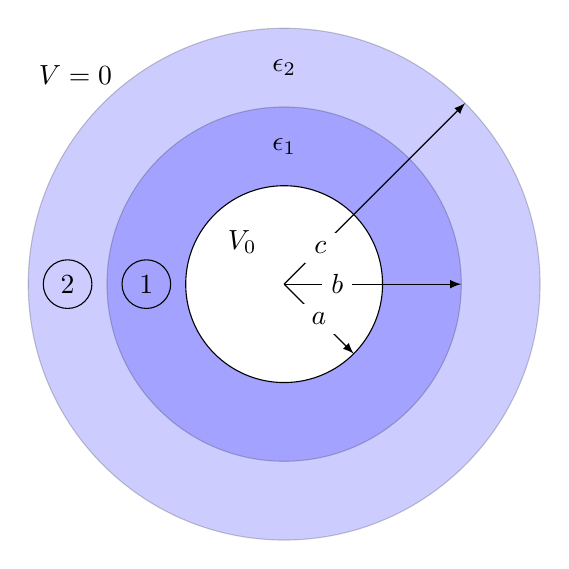
\begin{tikzpicture}
    \coordinate (O) at (0, 0);
    \edef\ra{3.25};
    \edef\rb{2.25};
    \edef\rc{1.25};

    \draw[fill=blue, opacity=.2] (O) circle (\ra);
    \draw[fill=blue, opacity=.2] (O) circle (\rb);
    \draw[fill=white] (O) circle (\rc);
    
    \node[draw, circle] at (-\ra/2-\rb/2, 0) {2};
    \node[draw, circle] at (-\rb/2-\rc/2, 0) {1};

    \node at (0, \ra/2+\rb/2) {$\epsilon_2$};
    \node at (0, \rb/2+\rc/2) {$\epsilon_1$};
  
    \draw[-latex] (O) -- ++ ({sqrt(\ra*\ra/2)}, {sqrt(\ra*\ra/2)}) node[pos=.2, fill=white] {$c$};
    \draw[-latex] (O) -- ++ (\rb, 0) node[pos=.3, fill=white] {$b$};
    \draw[-latex] (O) -- ++ ({sqrt(\rc*\rc/2)}, -{sqrt(\rc*\rc/2)}) node[pos=.5, fill=white] {$a$};

    \node[xshift=-10, yshift=10] at (-{sqrt(\ra*\ra/2)}, {sqrt(\ra*\ra/2)}) {$V=0$};
    \node[xshift=10, yshift=-10] at (-{sqrt(\rc*\rc/2)}, {sqrt(\rc*\rc/2)}) {$V_0$};

  \end{tikzpicture}
  \captionof{figure}{Estructura coaxial de \cref{q:coax}.}
  \label{fig:coax}
\end{center}


\begin{solution}
    \begin{parts}
    \part Al ser una estructura coaxial y no tener cargas ligadas ni cargas libres, resolveremos la ecuación de Laplace para coordenadas cilíndricas, es decir:
    \begin{equation}
    \nabla^{2}V = \frac{1}{r} \frac{\partial}{\partial r}\del{r \frac{\partial V}{\partial r}} + \frac{1}{r^{2}}\frac{\partial^{2}V}{\dif{\theta}^{2}} + \frac{\partial^{2}V}{\partial z^{2}}
  \end{equation}
    Notemos que estamos buscando  \(V(r)\), por ende, la ecuación a resolver se simplifica a lo siguiente:
    \begin{equation}
        \frac{1}{r} \frac{\partial}{\partial r}
        \left( r \frac{\partial V}{\partial r} \right) = 0
    \end{equation}
    Resolviendo:
    \begin{align}
        \frac{1}{r} \frac{\partial}{\partial r}
        \left( r \frac{\partial V}{\partial r} \right) &= 0 \\
        \frac{\partial}{\partial r}
        \left( r \frac{\partial V}{\partial r} \right) &= 0 \\
    \end{align}
    Por regla del producto:
    \begin{align}
        \frac{\partial r}{\partial r} \frac{\partial V}{\partial r}
         + r \frac{\partial^{2}V}{\partial r} &= 0 \\
         \frac{\partial V}{\partial r}
         + r \frac{\partial^{2}V}{\partial r^{2}} &= 0 \\
         \frac{\partial V}{\partial r} &= 
         -r \frac{\partial^{2}V}{\partial r}
    \end{align}
    Se puede hacer el siguiente cambio de variable: \\
    $u= \frac{\partial V}{\partial r} \\
    \frac{\partial u}{\partial r} = \frac{\partial^{2}V}{\partial r^{2}}$
    Así, nos queda:
    \begin{align}
        u &= -r\frac{\partial u}{\partial r} \\
        \frac{\partial u}{u} &= -\frac{\partial r}{r}
    \end{align}
    Integrando a ambos lados:
    \begin{align}
        \int \frac{du}{u} &= -\int \frac{dr}{r} \\
        \ln{u} &= -\ln{r} + C \\
        \exp{(\ln{u})} &= \exp{(-\ln{r} + C)} \\
        \exp{(\ln{u})} &= \exp{(\ln{\frac{1}{r}})} \cdot \exp{(C)}
    \end{align}
    Definiendo la constante $A=\exp{(C)}$:
    \begin{align}
        u &= A \cdot \frac{1}{r}
    \end{align}
    
    Reemplazando $u$ por $\frac{\partial V}{\partial r}$ (Revertir el cambio de variable), nos queda:
    \begin{align}
        \frac{\partial V}{\partial r} &= A \cdot \frac{1}{r} \\
        \partial V &= A \cdot \frac{\partial r}{r}
    \end{align}
    Se integra a ambos lados y se obtiene:
    \begin{align}
        V(r) &= A \cdot \ln{(r)} + B
    \end{align}
    Es importante tener en cuenta que al tener dos medios con permitividades distintas, se tienen dos soluciones (una para cada medio). Así, la solución para la ecuación de Laplace es: 
    \begin{align}
        V_1(r) &= A \cdot \ln{(r)} + B \\
        V_2(r) &= C \cdot \ln{(r)} + D
    \end{align}
    Ahora, para determinar las cuatro constantes se utilizarán ecuaciones ya conocidas y condiciones de borde. Por información del enunciado, tenemos que:
    \begin{align}
        V_1(r=a) &= A \cdot \ln{(a)} + B = V_0 \\
        V_2(r=c) &= B \cdot \ln{(c)} + D = 0
    \end{align}
    Además, por continuidad del potencial eléctrico, se cumplirá que $V_1(r=b) = V_2(r=b)$, es decir:
    \begin{align}
        A \cdot \ln{(b)} + B &= C \cdot \ln{(b)} + D
    \end{align}
    De esta manera, tenemos tres ecuaciones para cuatro incógnitas. La ultimá incógnita se obtendrá del campo eléctrico, que se relaciona con su potencial de la siguiente manera:
    \begin{align}
        E_{1}(r) &= -\nabla V_{1}=-\frac{A}{r} \uvec{r},   &  E_{2}(r) &= -\nabla V_{2}=-\frac{C}{r} \uvec{r}.
    \end{align}
    Por condición de borde:
    \begin{align}
        \epsilon_1 E^\bot_{1} - \epsilon_2 E^\bot_{2}
        =  D^\bot_{1} - D^\bot_{2} &= \upsigma_f
    \end{align}
    Dado que no hay carga libre, simplemente queda que:
    \begin{align}
        \epsilon_1 E^\bot_{1} &= \epsilon_2 E^\bot_{2} \\
        -\epsilon_1 \frac{A}{r} &= -\epsilon_2 \frac{C}{r} \\
        A &= C \frac{\epsilon_2}{\epsilon_1}
    \end{align} 
    De esta forma, a partir de las ecuaciones (23), (24), (25), y (30), podemos despejar las cuatro constantes y obtenemos lo siguiente:
    \begin{align}
      A&= \epsilon_{2}\del{-\frac{V_{0}}{\epsilon_{2}\ln\del{\frac{b}{a}} + \epsilon_{1}\ln\del{\frac{c}{b}}}}\\ 
      B &= V_{0} - A\ln(a)  = V_{0} + \frac{V_{0}\epsilon_{2}}{\epsilon_{2}\ln\del{\frac{b}{a}} + \epsilon_{1}\ln\del{\frac{c}{b}}}\\ 
      C &=  \frac{\epsilon_{1}A}{\epsilon_{2}} =\epsilon_{1}\del{-\frac{V_{0}}{\epsilon_{2}\ln\del{\frac{b}{a}} + \epsilon_{1}\ln\del{\frac{c}{b}}}}\\ 
      D&=-\frac{\epsilon_{1}A}{\epsilon_{2}} \ln(c) = \epsilon_{1}\del{-\frac{V_{0}}{\epsilon_{2}\ln\del{\frac{b}{a}} + \epsilon_{1}\ln\del{\frac{c}{b}}}}\ln(c)
    \end{align}
    Finalmente, obtenemos los potenciales y los campos eléctricos en ambos medios:
    \begin{align}
      V_{1}(r) &=  A\ln(r) + B =  \epsilon_{2}\del{-\frac{V_{0} }{\epsilon_{2}\ln\del{\frac{b}{a}} + \epsilon_{1}\ln\del{\frac{c}{b}}}} \ln(r) + V_{0} + \frac{V_{0}\epsilon_{2}}{\epsilon_{2}\ln\del{\frac{b}{a}} + \epsilon_{1}\ln\del{\frac{c}{b}}} \\
      V_{2}(r) &= C\ln(r) + D =\epsilon_{1}\del{-\frac{V_{0}}{\epsilon_{2}\ln\del{\frac{b}{a}} + \epsilon_{1}\ln\del{\frac{c}{b}}}} \ln(r)+\epsilon_{1}\del{-\frac{V_{0}}{\epsilon_{2}\ln\del{\frac{b}{a}} + \epsilon_{1}\ln\del{\frac{c}{b}}}}\ln(c) \\
      E_{1}(r) &= -\nabla V_{1} = \frac{V_{0}\epsilon_{2}}{\epsilon_{2}\ln\del{\frac{b}{a}} + \epsilon_{1}\ln\del{\frac{c}{b}}} \frac{1}{r}(\uvec{r}) \\
      E_{2}(r) &= -\nabla V_{2} =  \epsilon_{1}\del{\frac{V_{0}}{\epsilon_{2}\ln\del{\frac{b}{a}} + \epsilon_{1}\ln\del{\frac{c}{b}}}} \frac{1}{r} (\uvec{r})
    \end{align}

    \part Se busca obtener la carga total ${Q}$ en cada una de las placas de los electrodos. Al ser un condensador, ambas placas deberán tener en magnitud la misma carga, pero de signos opuestos. Así, por Ley de Gauss en forma integral:
    \begin{align}
        \iint \mathbf{E_1} \cdot \dif{a} &= 
        \iiint \frac{\rho}{\epsilon_1} \cdot \dif{\tau} = \frac{Q_{enc}}{\epsilon_1}
    \end{align}
    Así, podemos despejar la carga:
    \begin{align}
        Q_{1enc} &= \epsilon_1 \iint \mathbf{E_1} \cdot \dif{A} \\
        Q_{1enc} &= \epsilon_1 \iint \mathbf{E_1} \cdot a\dif{\theta}\dif{z} \\
        Q_{1} &= \epsilon_1 \iint \frac{V_{0}\epsilon_{2}}{\epsilon_{2}\ln\del{\frac{b}{a}} + \epsilon_{1}\ln\del{\frac{c}{b}}} \frac{1}{a} \cdot a\dif{\theta}\dif{z} \\
        Q_{1} &= \frac{\epsilon_{1}\epsilon_{2}V_{0}  2\pi d}{\epsilon_{2}\ln\del{\frac{b}{a}} + \epsilon_{1} \ln\del{\frac{c}{b}}}.
    \end{align}
    Para $Q_{2}$ el proceso es análogo, imponiendo el signo negativo propio del condensador, obteniendo la siguiente expresión:

\begin{align}
  Q_2 &= -\frac{\epsilon_{1}\epsilon_{2}V_{0}  2\pi d}{\epsilon_{2}\ln\del{\frac{b}{a}} + \epsilon_{1}\ln\del{\frac{c}{b}}}
\end{align}
Finalmente, se puede concluir que la carga es ambos electródos tiene igual magnitud pero distinto signo.

\part Se busca obtener la energía asociada al campo \textbf{E} en cada medio dieléctrico, lo cual vendrá dada por lo siguiente expresión matemática:
  \begin{align}
    w_{e} = \frac{1}{2} \epsilon E^{2}\del{r}.
  \end{align}
  Dada la expresión se observa que esta dependerá de cada medio en el cual estemos evaluando, por tanto haremos la división para cada medio. Recordemos que el campo eléctrico era:
  \begin{equation}
    \mathbf{E}_{1}(r) = \frac{-A}{r}\uvec{r}.
  \end{equation}
  Luego reemplazando en la ecuación de energía se obtiene:
  \begin{align}
    w_{e1} &= \frac{1}{2}\frac{\epsilon_{1}A^{2}}{r^{2}}.
  \end{align}
  Con lo que integrando sobre todo el volumen se tendrá que la energía total:
  \begin{align}
    W_{e1} &=\int_{v} w_{e1}dv =\int_{0}^{d}  \int_{0}^{2\pi} \int_{a}^{b}\frac{A^{2}}{r^{2}} \frac{1}{2}\epsilon_{1} \dif{r}(r \dif{\theta})\dif{z} = A^{2} \pi d\epsilon_{1} \int_{a}^{b} \frac{1}{r} \dif{r}= A^{2}\pi  d \ln\del{\frac{b}{a}} \epsilon_{1}.
  \end{align}
  Análogamente para el otro medio se obtendrá que:
  \begin{align}
    W_{e2}= C^{2} \pi d \ln\del{\frac{c}{b}} \epsilon_{2}
  \end{align}

  \part Nos dicen que $\vec{\mathbf{E_1}} = -\frac{A}{r}\hat{\mathbf{r}} + K_1\cdot\frac{\sin{(\theta)}}{r} \cdot \hat{\mathbf{\theta}}-K_2 z \cdot \hat{\mathbf{z}}$. Para verificar que el campo es conservativo, hay que encontrar un potencial tal que $\vec{\mathbf{E_1}}= -\nabla V$. Hay que notar que al estar en una simetría coaxial, se utilizará el gradiente en coordenadas cilíndricas, tal que:
  \begin{align}
      \vec{\mathbf{E_1}} &= -\nabla V = -\frac{\partial V}{\partial r}\,\hat{\mathbf{r}} - \frac{1}{r} \frac{\partial V}{\partial \theta}\,\hat{\mathbf{\mathbf{\theta}}} - \frac{\partial V}{\partial z}\,\hat{\mathbf{z}}
    \end{align}
    De esta manera, igualando $\vec{\mathbf{E_1}}$ con el gradiente del potencial se obtiene el siguiente set de ecuaciones diferenciales:
    \begin{align}
        \frac{\partial V}{\partial r} &= \frac{A}{r} \\
        \frac{1}{r} \frac{\partial V}{\partial \theta} &= -K_1 \cdot \frac{\sin{(\theta)}}{r} \\
        \frac{\partial V}{\partial z} &= K_2 z
    \end{align}
    Para encontrar el potencial, iniciamos resolviendo la primera EDO:
    \begin{align}
        \frac{\partial V}{\partial r} &= \frac{A}{r} \\
        \dif{V} &= A\cdot \frac{\dif{r}}{r}
    \end{align}
    Integrando a ambos lados:
    \begin{align}
        \int\dif{V^*} &= \int A\cdot \frac{\dif{r}}{r} \\
        V^* = A\cdot \ln{(r)} + f_{\theta, z}
    \end{align}
    Es importante notar que la constante de integración es una función dependiente tanto de $\theta$ como de $z$. A partir de aquí utilizaremos las otras dos EDOS para despejar esta función. Ahora con la segunda EDO:
    \begin{align}
        \frac{1}{r} \frac{\partial V}{\partial \theta} &= -K_1 \cdot \frac{\sin{(\theta)}}{r}
    \end{align}
    Pero utilizaremos $V^*$ para poder despejar la función incógnita, tal que:
    \begin{align}
        \frac{1}{r} \frac{\partial V^*}{\partial \theta} &= -K_1 \cdot \frac{\sin{(\theta)}}{r} \\
        \frac{1}{r} \frac{\partial (A\cdot \ln{(r)} + f_{\theta, z})}{\partial \theta} &= -K_1 \cdot \frac{\sin{(\theta)}}{r} \\
        \frac{\partial f_{\theta , z}}{\partial\theta} &= -K_1 \cdot \sin{(\theta)} \\
        \dif{f_{\theta , z}} &= -K_1 \cdot \sin{(\theta)} \dif{\theta} \\
        \int\dif{f_{\theta , z}} &=\int -K_1 \cdot \sin{(\theta)} \dif{\theta} \\
        f_{\theta , z} &= -K_1 \cdot (-\cos{(\theta)}) + f_z \\
        f_{\theta , z} &= K_1 \cdot \cos{(\theta)} + f_z
    \end{align}
    Ahora que encontramos una expresión para $f_{\theta , z}$, reemplazamos esta en nuestro potencial $V^*$:
    \begin{align}
  V^* &= A\cdot \ln{(r)} + K_1 \cdot \cos{(\theta)} + f_z
    \end{align}
    Repetimos el proceso para encontrar $f_z$ utilizando la tercera EDO:
    \begin{align}
        \frac{\partial V^*}{\partial z} &= K_2 \cdot z \\
  \frac{\partial (A\cdot \ln{(r)} + K_1 \cdot \cos{(\theta)} + f_z)}{\partial z} &= K_2 \cdot z \\
        \frac{\partial f_z}{\partial z} &= K_2 \cdot z \\
        \dif{f_z} &= K_2 \cdot z \dif{z} \\
        \int \dif{f_z} &= \int K_2 \cdot z \dif{z} \\
        f_z &= K_2 \cdot \frac{z^2}{2} + C
    \end{align}
    Y de esta forma, el potencial encontrado es:
    \begin{align}
  V^* &= A\cdot \ln{(r)} + K_1 \cdot \cos{(\theta)} + K_2 \cdot \frac{z^2}{2} + C
    \end{align}
    De esta forma, se encontró un potencial que cumple con la ecuación $\vec{\mathbf{E_1}}= -\nabla V^*$, por lo tanto, el campo eléctrico es conservativo.
    
    
      
    \end{parts}
\end{solution}

\question \label{q:rot_cyl} Un cilindro muy largo de radio R y densidad de carga volumétrica $\rho$ gira alrededor de su eje con frecuencia angular $\omega$. 
\begin{parts}
    \part Encuentre el campo magnético en algún punto sobre el eje de simetría del cilindro (eje z). 
    \part ¿Cómo cambia la respuesta si la carga estuviera depositada solo en la superficie del cilindro?

\end{parts}


\begin{center}
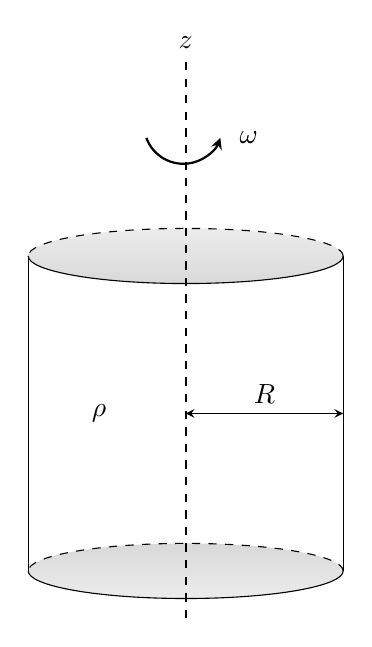
\begin{tikzpicture}[scale=1, >=stealth]
  % parámetros (ajusta \R y \H si quieres)
  \def\R{2}   % radio (unidades TikZ, p.ej. cm)
  \def\H{4}   % altura visible

  % auxiliar: altura intermedia para colocar la marca de R
  \pgfmathsetmacro{\ym}{0.5*\H}

  % --- elipses superior e inferior (sombreado para dar volumen) ---
  \shade[top color=gray!15,bottom color=gray!30] (0,\H) ellipse (\R cm and 0.35cm); % tapa (vista)
  \shade[top color=gray!30,bottom color=gray!15] (0,0) ellipse (\R cm and 0.35cm);  % base (vista)

  % --- paredes verticales ---
  \draw (-\R,0) -- (-\R,\H);
  \draw (\R,0)  -- (\R,\H);

  % --- arcos de la base (frente sólido, parte trasera punteada) ---
  \draw (-\R,0) arc (180:360:\R cm and 0.35cm);   % arco frontal (visible)
  \draw[dashed] (\R,0) arc (0:180:\R cm and 0.35cm); % arco trasero (oculto)

  % --- arcos de la tapa (frente sólido, trasero punteado) ---
  \draw (-\R,\H) arc (180:360:\R cm and 0.35cm);   % frente tapa (visible)
  \draw[dashed] (\R,\H) arc (0:180:\R cm and 0.35cm); % trasera tapa (oculta)

  % --- eje z (punteado) ---
  \draw[dashed,thick] (0,-0.6) -- (0,\H+2.5) node[above] {$z$};

  % --- marca del radio R desde el eje ---
  \draw[<->] (0,\ym) -- (\R,\ym) node[midway,above] {$R$};

  % etiqueta breve
  \node at (-1.1,\ym) {$\rho$};
  \draw[->,thick] (-1,\H+1.5) ++(0.5,0) arc (200:340:0.5cm);
  \node at (0.8,\H+1.5) {$\omega$};

\end{tikzpicture}
\captionof{figure}{Cilindro cargado de radio R, que rota con velocidad angular $\omega$ de la \cref{q:rot_cyl}.}
  \label{fig:rot_cyl}
\end{center}


\begin{solution}
\begin{parts}
    \part Usaremos Ley de Ampère (magnetoestática):
    \begin{align}
        \nabla \times \mathbf{B} &= \mu_0 \cdot \mathbf{J}
    \end{align}
    Por Teorema de Stokes, si integramos a ambos lados en una superficie cerrada, se obitene la Ley de Ampère en su forma integral:
    \begin{align}
        \iint\nabla \times \mathbf{B} \dif{a} &= \iint\mu_0 \cdot \mathbf{J} \dif{a} \\
        \int \mathbf{B} \cdot \dif{l} &= \mu_0\iint \mathbf{J} \cdot \dif{a}
    \end{align}
    Pero falta la densidad de corriente ($\vec{\mathbf{J}}$). Cuando tengamos ejercicios con figuras que rotan y velocidad angular dada, utilizaremos lo siguiente:
    \begin{align}
        \vec{\mathbf{J}} &= \rho \cdot \vec{v}
    \end{align}
    Donde $\vec{v}$ se puede expresar como:
    \begin{align}
        \vec{v}&= \vec{\omega} \times \vec{r} \\
        \vec{v}&= \omega \hat{z} \times r\hat{r} \\
        \vec{v}&= \omega r \hat{\theta}
    \end{align}
    Así, tenemos que:
    \begin{align}
        \vec{\mathbf{J}} &= \rho \cdot \vec{v} \\
        \vec{\mathbf{J}} &= \rho \omega r \hat{\mathbf{\theta}}
    \end{align}
    Ahora, podemos utilizar la Ley de Ampère y obtener el campo magnético:
    \begin{align}
        \int \mathbf{B} \cdot \dif{l} &= \mu_0\iint \mathbf{J} \cdot \dif{a}
    \end{align}
    Por un lado, la densidad de corriente tiene dirección $\mathbf{\hat{\theta}}$ (se asemeja a una bobina), por ende, el diferencial de superficie será el que va en $\mathbf{\hat{z}}$, es decir, $\dif{r} \cdot \dif{z} \cdot \mathbf{\hat{\theta}}$.  Por otro lado, el campo magnético irá en $\mathbf{\hat{z}}$ por regla de la mano derecha (ya que la corriente va en $\mathbf{\hat{\theta}}$),  y de esta forma el diferencial de línea será $\dif{z} \mathbf{\hat{z}}$. Así, la ecuación nos queda:
    \begin{align}
        \int \mathbf{B} \cdot \dif{z} \mathbf{\hat{z}} &= \mu_0\iint \mathbf{J} \cdot \dif{r} \cdot \dif{z} \cdot \mathbf{\hat{\theta}} \\
        \int \mathbf{B} \cdot \dif{z} \mathbf{\hat{z}} &= \mu_0\iint \rho \omega r \hat{\mathbf{\theta}} \cdot \dif{r} \cdot \dif{z} \cdot \mathbf{\hat{\theta}} \\
        \mathbf{B} \cdot l \mathbf{\hat{z}} &= \mu_0 \rho \omega l \int r \dif{r} \\
        \mathbf{\vec{B}} &= \mu_0 \rho \omega \frac{R^2}{2}\cdot \mathbf{\hat{z}}
    \end{align}
    Notemos que el campo no depende de $r$, es decir, es constante al interior del cilindro. Es por esto que el campo en cualquier punto sobre el eje de simetría (y en cualquier punto al interior del cilindro en realidad), es $\mu_0 \rho \omega \frac{R^2}{2}\cdot \mathbf{\hat{z}}$. \\
    Además, el campo al interior de un cilindro que rota es análogo al campo al interior de una bobina. Esto se debe a que la rotación del cilindro genera que la corriente tenga dirección en $\mathbf{\hat{\theta}}$, similar a las espiras enrolladas de un solenoide (pueden hacer el ejercicio y comparar). 

    \part Si tomamos carga solo en la superficie del cilindro, es decir, una densidad de carga $\mathbf{\sigma}$, estaríamos encerrando la misma cantidad de corriente. Por ende, el resultado no cambia.

    \end{parts}
    \end{solution}

\question Un conductor esférico de radio $r_a$, transporta una carga $Q$. El conductor es rodeado por un material dieléctrico lineal de susceptibilidad $\chi_e$ hasta a un radio $r_b$ (desde el centro del conductor esférico). Hallar la energía de esta configuración. Recuerde que la energía está expresada por:
  \begin{equation}
    W = \frac{1}{2}\int\mathbf{D}\cdot\mathbf{E}\dif\uptau
    \label{eq:work}
  \end{equation}

  \begin{solution}
    Comenzamos por calcular $\mathbf{E}$ y $\mathbf{D}$. Podríamos calcular $\mathbf{P}$, pero no conocemos $\mathbf{E}$. Afortunadamente sabemos el valor de la carga total $Q$, y usamos simetría esférica, entonces:
    \begin{equation}
      \mathbf{D} = \frac{Q}{4\pi r^2}\widehat{\mathbf{r}}, \quad\forall r>r_a.
    \end{equation}
    Dentro de la esfera metálica, al ser un material conductor, se tiene solamente carga en la superficie. Así, $\mathbf{E}=\mathbf{D}=\mathbf{P}=0$. Como $\mathbf{D}$ es \textit{proporcional} a $\mathbf{E}$, $\mathbf{D} = \epsilon\mathbf{E}$, podemos calcular el campo eléctrico en todo $\widehat{\mathbf{r}}$,
    \begin{equation}
      \mathbf{E} = \begin{cases}
        \frac{Q}{4\pi\epsilon r^2}\widehat{\mathbf{r}}, \quad r_a<r<r_b, \\
        \frac{Q}{4\pi\epsilon_0 r^2}\widehat{\mathbf{r}} \quad r>r_b.
      \end{cases}

    \end{equation}

    Donde $\epsilon   = \epsilon_0 (1+\chi_e)$ para la región con susceptibilidad $\chi_e$. Finalmente calculamos la Ec.~\eqref{eq:work},
    \begin{align}
      W &= \frac{1}{2}\int\mathbf{D}\cdot\mathbf{E}\dif\uptau = \frac{1}{2}\frac{Q^2}{\del{4\pi}^2}\times4\pi \del{ \frac{1}{\epsilon}\int_{r_a}^{r_b} \frac{1}{r^4}r^2\dif{r} + \frac{1}{\epsilon_0}\int_{r_b}^\infty \frac{\dif{r}}{r^2} } \\
      &= \frac{Q^2}{8\pi} \sbr{ \frac{1}{\epsilon}\eval{\del{-\frac{1}{r}}}^{r_b}_{r_a} + \frac{1}{\epsilon_0}\eval{\del{-\frac{1}{r}}}_{r_b}^\infty} = \frac{Q^2}{8\pi\epsilon_0}\sbr{\frac{1}{1+\chi_e}\del{\frac{1}{r_a} - \frac{1}{r_b}}+\frac{1}{r_b}} \\
      &= \frac{Q^2}{8\pi\epsilon_0\del{1+\chi_e}} \del{\frac{1}{r_a} + \frac{\chi_e}{r_b}}
    \end{align}
  \end{solution}
\end{questions}
\end{document}